\documentclass{standalone}
\usepackage{chez}

\begin{document}
\chapter{September 30, 2020}

\begin{definition}
  Let \(\mathcal C\) be a category and let
  \[
    \begin{tikzcd}
      A \arrow[r, "f"] \arrow[d, "g"'] &
        B \\
      C
    \end{tikzcd}
  \]
  be a diagram in \(\mathcal C\).
  A \vocab{pushout} of this diagram is a commuting square
  \[
    \begin{tikzcd}
      A \arrow[r, "f"] \arrow[d, "g"'] &
        B \arrow[d, "p_B"] \\
      C \arrow[r, "p_C"'] & P
    \end{tikzcd}
  \]
  such that for any other commuting square
  \[
    \begin{tikzcd}
      A \arrow[r, "f"] \arrow[d, "g"'] &
        B \arrow[d, "p_B'"] \\
      C \arrow[r, "p_C'"'] & P'
    \end{tikzcd}
  \]
  there is a unique map \(p \colon P \to P'\) with \(p \circ p_C = p_C'\)
  and \(p \circ p_B = p_B'\).
\end{definition}

\subsection{Pushouts in \texorpdfstring{\(\cTop\)}{Top}}
Suppose
\(
  \begin{tikzcd}[cramped, column sep=small, row sep=scriptsize]
    A \arrow[r, "f"] \arrow[d, "g"'] &
      B \\
    C
  \end{tikzcd}
\)
is a diagram in \(\cTop\).
Then the pushout
\[
  \begin{tikzcd}
    A \arrow[r, "f"] \arrow[d, "g"'] &
      B \arrow[d, "p_B"] \\
    C \arrow[r, "p_C"'] & P
  \end{tikzcd}
\]
has \(P = (B \sqcup C) / (\text{\(f(a) = g(a)\) for all \(a \in A\)})\),
where \(p_B \colon B \to P\) is the composite of the natural inclusion
and the quotient map \(B \to B \sqcup C \to P\).

\begin{example}
  The pushout of
  \(
    \begin{tikzcd}[column sep=scriptsize]
      C & \nullset \ar[l] \ar[r] & B
    \end{tikzcd}
  \)
  is just the disjoint union \(B \sqcup C\).
\end{example}

\begin{example}
  The pushout of
  \(
    \begin{tikzcd}[column sep=scriptsize]
      * & A \ar[l] \ar[r, "f"] & B
    \end{tikzcd}
  \)
  is the quotient \(P = B / \img f\).
\end{example}


\begin{definition}
  If there is a pushout square
  \[
    \begin{tikzcd}
      \coprod_{i \in I} S^{n-1} \arrow[r] \arrow[d, hook] &
        B \arrow[d] \\
      \coprod_{i \in I} D^n \arrow[r] &
        P
    \end{tikzcd}
  \]
  then we say that \(P\) is obtained from \(B\) by attaching \(n\)-cells.
\end{definition}
The idea is that we take \(B\), and find copies of \(S^{n-1}\) inside \(B\).
At those points, we glue copies of \(D^n\) such that the boundary of
the disks are the copies of \(S^{n-1}\) we selected.

\begin{example}
  The following pushout
  \[
    \begin{tikzcd}
      S^1 \sqcup S^1 \arrow[r] \arrow[d] &
        * \arrow[d] \\
      D^2 \sqcup D^2 \arrow[r] &
        P
    \end{tikzcd}
  \]
  is obtained from the point by attaching two \(2\)-cells.
  Geometrically, P looks like this:
  \begin{center}
    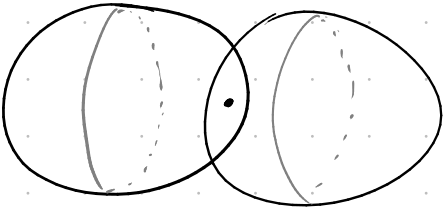
\includegraphics[width=0.25\textwidth]{18_905-200930-1.png}
  \end{center}
\end{example}
\begin{example}
  \begin{center}
    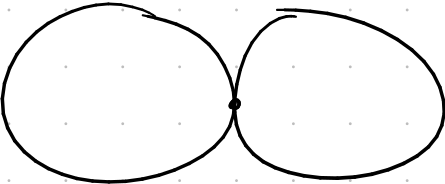
\includegraphics[width=0.2\textwidth]{18_905-200930-2.png}
  \end{center}
  The example one dimension lower is the figure-8 space,
  which is obtained from attaching two \(1\)-cells to a point, i.e.
  \[
    \begin{tikzcd}
      S^0 \sqcup S^0 \arrow[r] \arrow[d] &
        * \arrow[d] \\
      D^1 \sqcup D^1 \arrow[r] &
        P_8
    \end{tikzcd}
  \]
\end{example}

Another way to describe the figure-8 space \(P_8\)
is to say that it is homeomorphic to
\begin{center}
  \begin{tikzpicture}[scale=2]
    \begin{scope}[decoration={markings, mark=at position 0.5 with {\arrow{>}}}]
      \draw[postaction={decorate}] (1, 0) -- (1, 1) node[midway, right]{\(a\)};
      \draw[postaction={decorate}] (0, 0) -- (0, 1) node[midway, left ]{\(a\)};
    \end{scope}
    \begin{scope}[decoration={markings, mark=at position 0.5 with {\arrow{>>}}}]
      \draw[postaction={decorate}] (0, 0) -- (1, 0) node[midway, below]{\(b\)};
      \draw[postaction={decorate}] (0, 1) -- (1, 1) node[midway, above]{\(b\)};
    \end{scope}

    \fill (0, 0) circle[radius=0.02];
    \fill (0, 1) circle[radius=0.02];
    \fill (1, 0) circle[radius=0.02];
    \fill (1, 1) circle[radius=0.02];
  \end{tikzpicture}
\end{center}
where the square is not filled in.
Then, we see that there is a continuous map \(r \colon S^1 \to P_8\)
called \(a b a\inv b\inv\).
We can glue a \(2\)-cell to \(P_8\) by using \(r\) as the boundary.
\[
  \begin{tikzcd}
    S^1 \arrow[r, "r"] \arrow[d, hook] &
      P_8 \arrow[d] \\
    D^2 \arrow[r] & P
  \end{tikzcd}
\]
However, this just fills in the square,
so what we get is the torus \(P = T^2\).

\begin{definition}
  A \vocab{CW complex} \(X\) is a space with a sequence of subspaces
  \[
    \nullset = \Sk_{-1} X
      \subseteq \Sk_0 X
      \subseteq \Sk_1 X
      \subseteq \Sk_2 X
      \subseteq \dots \subseteq X
  \]
  such that
  \begin{itemize}
    \item \(X\) is the union of its \vocab{skeleta} \(\Sk_n X\)
    \item there exist pushout diagrams
    \[
    \begin{tikzcd}
      \coprod_{i \in I_n} S^{n-1} \arrow[r] \arrow[d, hook] &
        \Sk_{n-1} X \arrow[d] \\
      \coprod_{i \in I_n} D^n \sqcup D^1 \arrow[r] &
        \Sk_n X
    \end{tikzcd}
    \]
    i.e.\ \(\Sk_n X\) is obtained from \(\Sk_{n-1} X\)
    by attaching \(n\)-cells.
  \end{itemize}
\end{definition}

\begin{remark}
  Tomorrow is October so we can start talking about skeletons.
\end{remark}

\begin{example}
  The torus \(T^2\) can be given the structure of a CW complex with
  \begin{align*}
    \Sk_0 T^2 &= * \\
    \Sk_1 T^2 &= P_8 \\
    \Sk_2 T^2 &= T \\
    \Sk_3 T^2 &= T. \\
    \MTFlushSpaceAbove
    &\vdotswithin{=}
  \end{align*}
\end{example}

\begin{definition}
  A CW-complex is \vocab{finite dimensional} if \(\Sk_n X = X\) for some \(n\).
  The \vocab{dimension} of \(X\) is the smallest \(n\) for which this is true.
\end{definition}

This means that \(T^2\) is two dimensional.
However, a generic CW complex may he infinite-dimensional.

\begin{definition}
  A CW complex is of \vocab{finite type} if each \(I_n\) is finite.
\end{definition}

\begin{definition}
  A CW complex is \vocab{finite} if
    it is finite dimensional
    and of finite type.
\end{definition}

Here are some facts from point set topology that
we will not check, but are true.
\begin{lemma}
  \begin{itemize}[nosep]
    \item Any CW complex is Hausdorff.
    \item A CW complex \(X\) is compact if and only if \(X\) is finite.
    \item Any compact smooth manifold can be given some finite
      CW complex structure.
  \end{itemize}
\end{lemma}

Note that we can organize CW complexes into a category \(\cCWcomp\) where
the morphisms are diagrams
\[
  \begin{tikzcd}[row sep=small]
  	\vdots & \vdots \\
  	\Sk_{n+1} X \ar[r] \ar[u, symbol=\subseteq]
      & \Sk_{n+1} Y \ar[u, symbol=\subseteq] \\
  	\Sk_{n} X \ar[r] \ar[u, symbol=\subseteq]
      & \Sk_{n} Y \ar[u, symbol=\subseteq] \\
  	\vdots  \ar[u, symbol=\subseteq]
      & \vdots  \ar[u, symbol=\subseteq] \\
  	\Sk_{0} X \ar[r] \ar[u, symbol=\subseteq]
      & \Sk_{0} Y \ar[u, symbol=\subseteq]
  \end{tikzcd}
\]

There is a functor
\[
  \mathcal U \colon \cCWcomp \to \cTop
\]
that ignores the skeletal structure and just returns the union of the skeleta.

There is also a functor
\[
  \Fun(\Deltainj^\op, \cSet) \to \cCWcomp
\]
where we consider the simplicial sets geometrically,
i.e.\ if \(X_\bullet\) is a simplicial set,
\(X_n\) is the set of \(n\)-cells in the corresponding CW complex,
and the \(d\) maps give the boundaries of the gluing.

The composite functor
\[
  \Fun(\Deltainj^\op, \cSet) \to \cCWcomp \overset{U}\to \cTop
\]
is called the \vocab{geometric realization}.

The goal is to understand \(H_n\) of a geometric realization.
In particular We want to confirm that the homology of
a semisimplicial set is the same as its geometric realization.

\begin{example}
  \(S^n\) can be given a CW structure with one \(0\)-cell and one \(n\)-cell.
  In particular, there is a pushout diagram
  \[
    \begin{tikzcd}
      S^{n-1} \arrow[r] \arrow[d, hook] &
        * \arrow[d] \\
      D^n \arrow[r] &
        S^n
    \end{tikzcd}
  \]
  However, we can form a different CW structure on \(S^n\):
  \begin{align*}
    \Sk_{-1} S^n &= \nullset \\
    \Sk_0 S_n &= * \sqcup * = S^0 \\
    \Sk_1 S_n &= S^1 \\
    \shortvdotswithin{=}
    \Sk_n S_n &= S^n \\
    \Sk_{n+1} S_n &= S^n \\
    \MTFlushSpaceAbove
    &\vdotswithin{=}
  \end{align*}
  where to get from \(\Sk_{k-1} S^n\) to \(\Sk_n S^n\),
  we glue two \(k\)-cells as ``hemispheres``.
\end{example}

Note that there is a CW complex \(S^\infty\) which has
\(\Sk_n S^\infty = S_n\) for all \(n\).
Note that \(S^\infty\) is of finite type, but is not finite.



\end{document}
